\documentclass[conference]{IEEEtran}
\usepackage[T1]{fontenc}
\usepackage{amsmath}
\usepackage{graphicx}
\usepackage{float}
\usepackage{enumitem}

\title{Capacitor Charging and a Power On Rest for an Active Low Microcontroller}
\author{
    \IEEEauthorblockN{Andrei Prodan}
    \IEEEauthorblockA{Department of Computer Engineering Technology\\Vanier College}
}

\begin{document}

\maketitle

\begin{figure}[H]
    \centering
    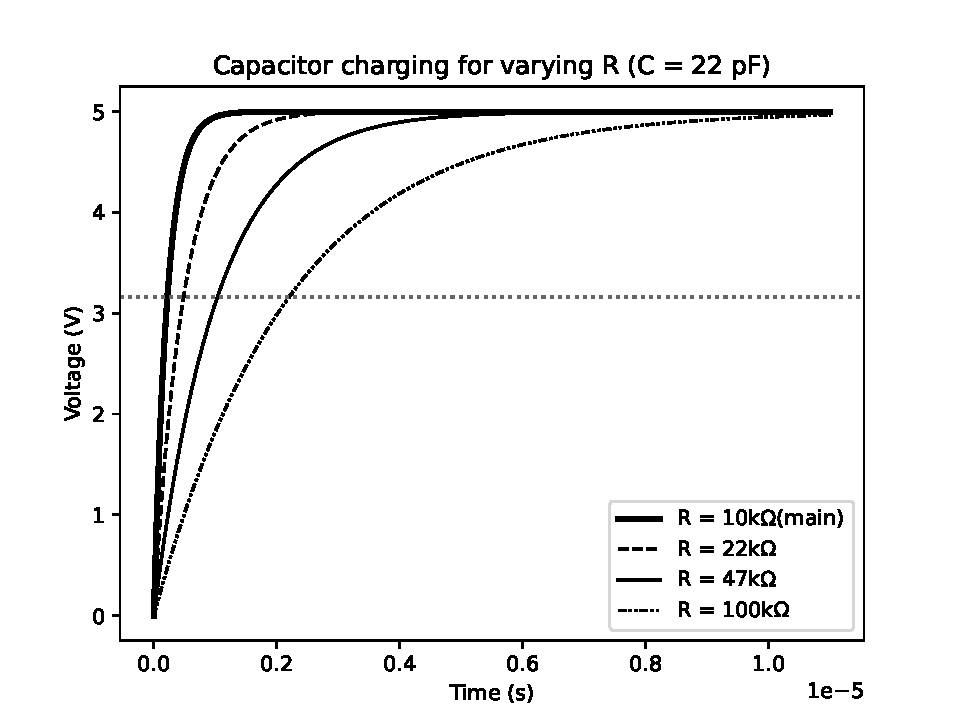
\includegraphics[width=\linewidth]{rc-charging2.pdf}
    \caption{Charging curves for four resistances, C = 22pF}
    \label{fig:1}
\end{figure}

\begin{abstract}
    This document derives the charging behaviour of a resistor-capacitor (RC) network, the voltage reached after one time constant, and applies the result to size a power-on-rest (POR) circuit for a microcontroller with an active-low reset.
\end{abstract}

\section{Introduction}
When a capacitor $C$ is charged through a series resistor $R$ from a constant supply $V_0$, the capacitor voltage rises according to

\begin{equation}
    V(t) = V_0(1-e^-t/RC),
    \label{equ:1}
\end{equation}

where $\tau =RC$ is the time constant. Substituting $t=\tau$ gives $V(\tau) = V_0(1-e^{-1})\approx0.632V_0.$

\section{Power On Reset with an Active Low Reset}
A power-on-reset circuit exploits \ref{equ:1} directly: $R$ from $V_{CC}$ to the reset node and $C$ from that node to ground hold the microcontroller's active-low reset pin low until the node crosses $V_{IH}$, releasing the device.

\begin{figure}[H]
    \centering
    
\includegraphics[width=0.5\linewidth]{por_circuit.pdf}
    \caption{Power-on-reset network driving an active-low reset pin}
    \label{fig:2}
\end{figure}

\subsection{Sizing R for a Timing Constraint}
The reset pin releases the instant the node voltage reached $V_{IH}$. Setting $V(t_{release}) = V_{IH}$ and solving for $t_{release}$:

\begin{equation}
    \begin{split}
    V_{IH} = V_0(1-e^{-t_{release}/RC})\\
    \frac{V_{IH}}{V_0} = 1-e^{-t_{release}/RC}\\
    e^{-t_{release}/RC} = 1-\frac{V_{IH}}{V_0}\\
    -\frac{t_{release}}{RC} = ln(1-\frac{V_{IH}}{V_0})\\
    t_{release} = -RCln(1-\frac{V_{IH}}{V_0})
    \label{equ:2}
    \end{split}
\end{equation}

Rearranging \ref{equ:2} for $R$, given a target $t_{release}$ and a chosen $C$:

\begin{equation}
    R = \frac{-t_{release}}{Cln(1-\frac{V_{IH}}{V_0})}
    \label{equ:3}
\end{equation}

\begin{enumerate}
    \item\textit{Worked example:} Take $V_{IH}=0.7V_0, V_0=5$V, and a target $t_{release}=10$ms. The $C = 22$pF used for the plots above was chosen only to keep the curves readable at a sub-microsecond timescale; a practical timing design instead starts from $C=100$nF. Evaluating the denominator of \ref{equ:3}:
    
    \begin{equation}
        ln(1-0.7) = ln(0.3)\approx-1.204.
    \end{equation}
    
    Substituting into \ref{equ:3}:

    \begin{equation}
        R = \frac{-(10\times10^{-3})}{(100\times10^{-9})\times(-1.204)}\approx83k\Omega.
    \end{equation}

    An $83k\Omega$ resistor with a 100nF capacitor gives a reset hold-off of approximately 10ms. Keeping C at the plotting value of
\end{enumerate}

\end{document}
